\documentclass[aps,  
                a4paper, 
                amsmath, 
                amssymb, 
                preprint,
                tightenlines,  
                amsfonts,
                nofootinbib,
                onecolumn,
                titlepage,
                10pt
            ]{revtex4-2}
\usepackage[utf8]{inputenc}
\usepackage{geometry, amsmath, amsthm, latexsym, amssymb, graphicx, amsfonts, blindtext, titlesec, xcolor}

\begin{document}

%\title{Improving the optomechanics of a BAW resonator for quantum amplification within future gravitational wave detectors}
%\author{Joseph Hocking\\\textbf{Supervisors:} Prof. C. Zhao, Prof. Ju Li}
%\noaffiliation
%\date{\today}

\begin{titlepage}
    \begin{center}
        %\vspace*{1cm}
            
        \Large
        \textbf{Improving the optomechanics of a BAW resonator for quantum amplification within future gravitational wave detectors}
            
        %\vspace{0.5cm}
        %\LARGE
        %Thesis Subtitle
            
        \vspace{1.5cm}
        
        \large
        \textbf{Joseph Hocking}\\
        \vspace{0.25cm}
        \textbf{Supervisors:} Prof. C. Zhao, Prof. Ju Li
            
        \vfill
            
        A Research Proposal for the degree of\\
        Master's in Experimental Physics
            
        \vspace{0.8cm}
            
        
\includegraphics[width=0.4\textwidth]{img/uwa-logo.png}
            
        \large
        ARC Centre of Excellence for Gravitational Wave Discovery\\
        Department of Physics\\
        University of Western Australia\\
        \today
            
    \end{center}
\end{titlepage}

\tableofcontents

\section{Introduction}
    \par
    Gravitational waves, ripples in the very fabric of space-time, were once thought to be the playground of theoretical physicists. A fun quirk falling out of Einstein's revolutionary theory of general relativity. That was until in September of 2015, when we first directly heard the rumblings of universe. A true testament to the hard work and utter dedication of over half a century of international collaboration. We are now on the cusp of a new era of astronomy, the era of gravitational wave detection. It was Feynman, in a conference in 1957, described the first gravitational wave detector (GWD) in a mock thought experiment. Imagine a rigid rod, with two beads freely sliding (with friction), as the gravity wave passes through the rod the rigidity of it does not allow it to move with the wave. However, the proper distance between the beads will move, and due to this some small amount of energy will be deposited within the system, energy from the wave itself. Thus a it was realised that, theoretically at the minimum, one could detect gravitational waves. It was quickly noted, however, that due to the incredible stiffness of space-time, there existed no such material that could resist the motion of the wave.
    \par
    The first experimental attempts at gravitational wave detections were through the use of \textit{Resonant Mass Antennas}. These consist of a large bar precisely machine to have a resonant frequency matching that of expected gravitional wave sources. These achieved sensitivies on the order of $10^{-19}\varepsilon/\sqrt{Hz}$, chiefly through the use of advanced seismic isolation systems, cryogenic cooling, and materials with extreme mechanical Q-factors. There were some who claimed (and some who still do) that these incredible experimental system did detect gravitional waves, see ref{ref:webber-detection}, but the consensus of the wider scientific community beleives that there simply were not sensitive enough.
    \begin{figure}[h]
        \centering
        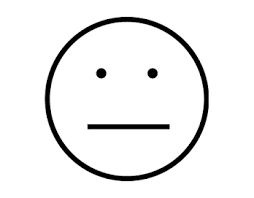
\includegraphics[width=0.5\textwidth]{img/blank.png}
        \caption{A simplified schemiatic of an inferometric gravitational wave observatory.}
        \label{fig:resonant_bar}
    \end{figure}
    \par
    The next generation of GWDs came in the form of large laser-based interferometers. The are a modified Michelson interferometer, with optical cavities within the arms. The end mirrors of the arms are tuned such that the phase of the two beams destructively interferes on the output (dark port) of the detector. When a gravitational wave passes through, differential stretching and squeezing of the two arms causes a phase difference in the beams, resulting in light at the output port. The current second generation interferometers, with newly implemented frequency dependent squeezing, are capple of reaching sensitivities of $10^{-24}\varepsilon/\sqrt{Hz}$. However, for events such as binary neutron star coalescence, much of the information about the progentor objects, the merger, and the resultant object is contain within the high frequencyu ring down above 1kHz. Unfortunately, current detectors are limited to peak sensitivities below 500Hz by quantum noise mechanisms.

\section{Quantum Amplification through White Light cavities}
    \subsection{Gravitational Wave Detector Noise}
    \label{sec:gwd-noise}
    The main categories of detector noise may be divided up into three rough frequency regimes. Within the \textbf{low frequency regime}, we are dominated by classical noise sources. This is largely related to the seismic motion of the ground coupling into the suspension system for the mirrors and so outside the scope of this work. In the \textbf{mid-frequency regime} we begin to see the radiation pressure back-action of the interferometer. Due to the quantum uncertainty of the photons' amplitude and arrival time, the radiation pressure exerted on the mirrors when they are reflected is noisy. As the interferometer is measuring the relative positions of the mirrors, this will become phase noise on the output and gives the radiation pressure noise seen within this frequency band. Finally, within the \textbf{high frequency regime}, we are limited by the quantum shot noise of the photons, or rather quantum uncertainty directly in the phase of the 
    photons.\footnote{Interestingly, this quantum noise does not in fact come from the bright port of the detector (where the laser is injected) as the quantum noise associated with this port will create in-phase noise down the two arms, while will be destructively interfered. Instead the quantum noise is associated with the dark port of the detector, where the beam splitter will serve to shift the noise to be out of phase between the two arms. This is why squeezing is performed on a vacuum state and injected into the dark port}
    It is important to note that this noise source is independent of the frequency of gravitational wave, however, it's effect on the strain senistivity of the detector is not. To see how this can be, we must examine the response of the detector within the frequency domain.
    \par
    The full detector is composed of many coupled cavities, however we will choose to simplify down to a single Fabry-Perot cavity with identical mirrors of power reflectivity $R$ and power transmission $T$. This will have a normalised intensity of light within the cavity, as a function of light frequency $\nu$, given by
    \begin{equation}
        \label{eq:fabry-perot-intracavity-intensity}
        I(\nu)=\frac{T}{1+R^4-2R\cos{(\Phi(\nu))}}, \qquad \Phi(\nu)=\frac{4\pi\nu L}{c}
    \end{equation}
    \begin{figure}
        \centering
        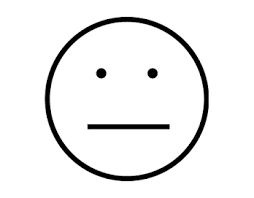
\includegraphics[width=0.5\textwidth]{img/blank.png}
        \caption{A spectrum of a Fabry-Perot cavity.}
        \label{fig:fabry-perot-spectrum}
    \end{figure}    
    Where $L$ is the length of the cavity arm, and $c$ is the speed of light. This is graphically shown in Fig \ref{fig:fabry-perot-spectrum}, in which one can observe that the lower frequency gravitational wave signals are amplified by the cavity, while the higher frequency signals will be damped. This reduces the photon count at these high frequencies which, due to the Poisson counting statistics of the photons, will lead to a high relative uncertainty. This is the root cause of the shot-noise related strain noise.
    \subsubsection*{Gain-Bandwidth Relationship}
    Moreover, assuming we are operating near the resonant frequency, that is the round-trip phase accumulation $\Phi(\nu_0)= 2n\pi$ for integer $n$, and the mirrors are near 100\% reflectivity, we can simplify \eqref{eq:fabry-perot-intracavity-intensity} down to
    \begin{equation}
        \label{eq:fabry-perot-resonance-intensity-simplified}
        I(\nu_0)\approx\frac{4}{T}
    \end{equation}
    Additionally, the resonance condition will be met every free spectral range (FSR), that is $\nu_{FSR}=c/2L$. And so for finesse $\mathcal{F}$ and cavity bandwidth $\nu_{FWHM}$ we have
    \begin{equation}
        \label{eq:FWHM-relationship}
        \nu_{FWHM}=\frac{\nu_{FSR}}{\mathcal{F}}=\frac{c/2L}{\pi r/(1-R)}\approx\frac{c/2L}{2\pi/T}\implies\nu_{FWHM}\propto T
    \end{equation}
    By examining \eqref{eq:FWHM-relationship} and \eqref{eq:fabry-perot-resonance-intensity-simplified}, we can see that the higher the gain, the lower the bandwidth. Thus we must either sacrafice on peak strain sensitivity for the sake of a larger bandwidth, or prioritise peak sensitivity over broadband sensitivity. Real GWDs are much more complicated than this, but the argument still remains the same. Ideally we would like to have a high gain, whilst maintaining a high bandwidth. This would be incredibly insightful into the the pre-merger and post-merger remnants of gravitational wave events, allowing us to see the full waveform of the in-spiral and merger. To do so, we must go beyond the classical physics described here.

    \subsection{White Light Cavities}
    In 1997, Whicht et al. proposed a concept, from herein referred to as a White Light Cavity or WLC, to utilize a quantum amplification scheme to break this gain-bandwidth relationship. The proposed scheme would introduce a medium into the signal recycling cavity that would correct the phase such that $\Phi(\nu)\approx n\pi$ for a large range of $\nu$, whilst maintaining the frequency shift induced by the gravitational wave. The corrected photons would then be fed back into the arm cavities for further amplification. Such a medium would be said to have an anomalous (also called negative) dispersion effect (AD or ND), that is the phase shift would be inversely proportional to frequency. This would, in effect, widen the bandwidth of the arm cavities whilst maintaining the same high gain. Mathematically, for carrier laser frequency $\omega_0$, the detectors arm length, $L_{arm}$, is tuned such that
    \begin{equation}
        \label{eq:cavity-resonance-condition}
        \frac{\omega_0L_{arm}}{c} = n\pi, \qquad n\in\mathbb{Z}
    \end{equation}
    When a gravitational wave of frequency $\Omega$ couples into the detector, our signal now has a frequency $\omega_0+\Omega$, these photons will therefore experience a phase shift of $\phi_{shift}=2\Omega L_{arm}/c$. So ideally, our negative dispersion medium will have a frequency dependent phase shift of
    \begin{equation}
        \label{eq:phase-correction}
        \phi_{ND} = -\frac{2\Omega L_{arm}}{c}
    \end{equation}
    % TODO Add figure of the acc. phase and phase correction here
    AD is traditionally observed around strong absorption lines, so along with their proposal for the WLC scheme, Whicht et al. suggested that an atomic media, held near absorption by a pump beam, may create a sufficient negative dispersion effect, however it was later shown that, when implemented into a interferometric system, optical instability would place unrealistic constraints on the media, making it unsuitable for use within a WLC scheme. An alternative proposed method of inducing negative dispersion is through the use of an unstable optomechanical filter, this has been the focus of WLC research as of recently. There are three candidate optomechanical resonators that may be used to create the unstable filter:
    \begin{description}
        \item[Phononic Membrane] This is a small membrane made from a highly reflective crystal, which a lattice of holes punched into the surface such that they create a mechanical band gap that traps phonons within a defect in the lattice. This benefits from low mass and high mechanical Q factor, but suffers from large thermal heating due to its small heat capacity.
        \item[Micro-Resonators] Micron-scale suspended mirrors, which utilise a pendulum mode for the mechanical motion. There are two types with this category: the Cat-flap, which is a rectangular AlGaS pendulum, and the lollipop, which is a circular AlGaS pendulum.
        \item[Bulk Acoustic Wave (BAW) Resonator] This is the focus of this proposal, and will be explained in detail further on, but as a brief description: The BAW is a plano-convex quartz crystal that is able to form a bulk phonon wave, this allows for a large mechanical Q, and its relatively large mass is beneficial for reducing the effect of laser heating. The large mass, on the other hand, also results in low optomechanical coupling, requiring large amounts of laser power for sufficient negative dispersion to occur.
    \end{description}
    
    \subsection{Overview of ND through Optomechanical Resonators}
    For any optomechanical interaction, we may model it through a 3-mode interaction, which have an input-output relation of
    \begin{equation}
        \label{eq:3-mode-in-out}
        \hat{a}_{out}=\frac{\Omega+i(\gamma_m+\gamma_{opt})}{\Omega+i(\gamma_m-\gamma_{opt})}\hat{a}_{in} + \hat{n}_{th}
    \end{equation}
    Where our mechanical damping is given by $\gamma_m\equiv\omega_m/Q_m$, with $Q_m$ being the mechanical Q factor of our optomechanical filter. And our negative optomechanical damping is given by $\gamma_{opt}\equiv g^2/\gamma_f$, where $\gamma_f$ is the filter cavity bandwidth, and $g$ is the optomechanical coupling of the resonator. Included in this equation is the thermal noise term, $\hat{n}_{th}$, this will be ignored for now but will place further requirements on the resonator. Note that this only applies within the resolved sideband regime, that is, when $\omega_m\gg\gamma_f\gg\Omega$, for filter cavity bandwidth $\gamma_f$. Additionally, by operating as an unstable optomechanical filter, which by definition is the regime such that $\gamma_{opt}\gg\gamma_m$, we can make the following approximations
    \begin{equation}
        \label{eq:in-out-approx}
        \hat{a}_{out}\approx\frac{\Omega+i\gamma_{opt}}{\Omega-i\gamma_{opt}}\hat{a}_{in}\approx-\exp{\left(\frac{-2i\Omega}{\gamma_{opt}}\right)}\hat{a}_{in}
    \end{equation}
    That is, our output experiences a phase shift of $\phi=-2\Omega/\gamma_{opt}$ so to satisfy the requirements outlined in Eqn \eqref{eq:phase-correction}, we have
    \begin{align}
        \label{eq:gamma-opt-req}
        \gamma_{opt}&=\frac{2\Omega L_{arm}}{c}=\frac{g^2}{\gamma_f}, \qquad g^2=\left(\frac{d\omega}{dq}\right)^2x_{xpf}^2\bar{a}^2\\
        \label{eq:filter-power-req}
        \implies P_c&=2\frac{m\omega_m c \Omega L_{arm}}{\mathcal{F}\omega_0}
    \end{align}
    \textbf{\color{red} I cant seem to replicate this using Page 2021 and Ma 2015!}
    \par
    Additionally, we can examine the restrictions placed on the mechanical Q-factor of the resonator, $Q_m$, through the effect of thermal noise. $\hat{n}_{th}$ is uncorrelated with the input optical field, and so to make it such that the effect does not dominate over any benefit from the WLC scheme, we require that
    \begin{equation}
        \label{eq:thermal-noise}
        \frac{8k_BT_{envir}}{Q_m}<\hbar\gamma_{IFO}.
    \end{equation}
    %TODO Add figure of strain sensitivity at different T/Q
    Where $\gamma_{IFO}$ is the detector bandwidth prior to the implementation of the unstable filter, and $T_{envir}$ is the resonator temperature. This provides a convenient figure of merit for optomechanical filters to be used in the WLC scheme, $T/Q$. As an order of magnitude estimate, to maintain near the sensitivities of current generation interferometers, we require $T/Q\sim6\times10^{-10}K$. That is, if we operate our mechanical filter at 1K, we would require a mechanical Q factor of $6\times10^{10}$. 

    \subsubsection*{The BAW as an unstable optomechanical filter}
    Previous study on the feasibility of a BAW resonator within this role had been performed with Ref \cite{page2021}, in which the authors identified a nominal value for the peak coupling strength associated with the resonator adn thus inferred a minimum filter cavity power requirement. For a crystal, of refractive index $n_Q$, centre position $x_p=(x_1+x_2)/2$, and a crystal thickness $q$, held within a cavity of length $L_f$ and at resonant laser wave number $k$, then the resonance condition is given by:
    \begin{equation}
        \label{eq:page-BAW-resonance-condition}
        \frac{n_Q\tan[k(x_p-q/2)]-\tan[n_Qk(x_p-1/2)]}{1+n_Q\tan[k(x_p-q/2)]\tan[n_Qk(x_p-1/2)]}=\frac{n_Q\tan[k(x_p+q/2-L_f)]-\tan[n_Qk(x_p-1/2)]}{1+n_Q\tan[k(x_p-q/2)]\tan[k(x_p+q/2-L_f)]}
    \end{equation}
    Assuming a small motion of $q$, we can take $dw/dq$ to be linear and negative. For typical values of quartz, as described in Ref \cite{page2021}, we can expect to see a coupling of $d\omega/dq\approx2\pi\times0.018\text{GHz nm}^{-1}$ for a 20mm table top experiment as will be described in later sections of this proposal. For a realistic filter cavity length of 5cm, this coupling frops down to $2\pi\times0.0075\text{GHz nm}^{-1}$, which implies a filter cavity optical intensity requirement of $P_c\sim17\text{MW cm}^{-2}$. Theoretically, quartz and the AlGaAs coatings should withstand these high intesities, however it is unclear whether the laser heating within the quartz would breach the strict thermal noise requirements described above. This issue motivates the need to induce higher optomechanical coupling of the BAW resonator, through the application of reflective coatings onto the crystal, this would reduce the power requirement, but would also lead to a degraded mechanical Q factor of the resonator, and so requiring a balance to be found between these competing issues. This research proposal will seek to examine the relationship between the increase of coupling strength through the application of further silicon nitride coatings and the degradation of the mechanical Q-factor, along with experimental measurements of the radiation pressure excitement of mechanical modes of the BAW.

    \section{Previous Works}
    A forthcoming paper will discuss the experimental comparison of an uncoated BAW resonator ($R_m\approx4\%$) and a resonator coated with a single thin layer of silicon nitride ($R_m\approx16\%$). Firstly, a novel approach to simulating the coupling strength of a BAW resonator is presented, as well as a comparison of the theoretical predictions to the experimental results. These experimental measurements were made with the crystals placed within a $\sim20$mm cavity, whose length was scanned to map the resonances as the crystal position was actuated. 

    To simulate the coupling of the cavity, an approximation of the system was made to a double membrane in the middle (dMIM) cavity. This was made under the assumption that the optomehcanical interaction only occurs at the interfaces of the resonator, and not within the bulk structure of the crystal\footnote{This is approximately true within the MHz range, however Ref \cite{kharel2019} demonstrated high coupling through Brillouin scattering within the GHz regime, unfortunately these modes have too low of a Q-factor to be considered for a WLC scheme.}. A dMIM configuration within a cavity has already been well studied by Ref \cite{li2016}, which should the transmission of such a cavity is given by
    \begin{align}
        \label{eq:transmission-dmim}
        \mathcal{T}_c=\frac{(1-R)^2(1-R_m)^2}{\vert\mathcal{D}\vert^2},
    \end{align} 
    where
    \begin{align}
        \label{eq:transmission-dmim-denom}
        \vert\mathcal{D}\vert^2=A\chi^2(kL)+B\chi(kL)+C,
    \end{align}
    in which
    \begin{align}
        \chi(kL)&=\sin({kL})-R_m\sin{(kL-2kq)}\nonumber\\
        A&=4R\nonumber\\
        B&=8\sqrt{RR_m}(1+R)\cos{(2kQ)}\sin{(kq)}\nonumber\\
        C&=8RR_m\cos(4kQ)\sin^2(kq)-2R(1-R_m)^2+(1+R^2)[1-2R_m\cos(2kq)+R_m^2].
    \end{align}

    Where $q$, $Q\equiv x_p$ are the effective (that is, corrected for the refractive index of quartz) thickness and position of the resonantor. As before $k$ is the laser wavenumber, and $L$ is the cavity length. $R$ is the power reflectivity of the cavity mirrors, with $R_m$ being the power reflectivity of each surface of the BAW. Note that, unlike the analysis done in Ref \cite{li2016}, here the phase shift due to the coating is not considered due to the thinness of the single layer. These expressions are a generalisation of the understanding of coupling mechanism described in Ref \cite{page2021}, not only allowing for arbitrary reflectivities of the crystal interfaces, but also the analysis of two different modes of motion: position mode, where the position of the crystal is actuated, and thickness mode, where the thickness of the crystal is modulated. The transmission heatmap is shown in Figure \ref{fig:transmission-dmim}. 
    \begin{figure}
        \centering
        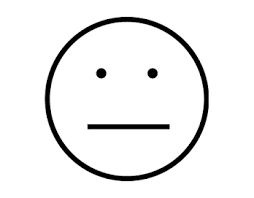
\includegraphics[width=0.5\textwidth]{img/blank.png}
        \caption{Simulated transmission of the BAW cavity.}
        \label{fig:sim-transmission-dmim}
    \end{figure}
    \par
    For experimental confirmation of these simulations, a BAW resonator was placed into an approximately $\sim20$mm long cavity. The length was scanned whilst actuating the postition of the crystal to map the resonaces of the position mode. This measurement was made for both an uncaoted resonator and the coated one. The transmission heatmap is shown in Figure \ref{fig:exp-transmission-dmim}. The experimental results were found to be in good agreement with the simulation's predictions.
    \begin{figure}
        \centering
        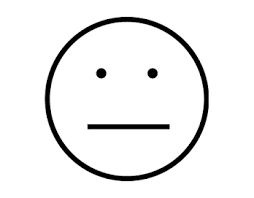
\includegraphics[width=0.5\textwidth]{img/blank.png}
        \caption{Experimental transmission of the BAW cavity.}
        \label{fig:exp-transmission-dmim}
    \end{figure}
    \par
    Now that the simulation's assumption have proved to be experimentally valid, the position mode was simulated and the gradient $d\omega/dq$ calculated in Fig \ref{fig:gradient-dmim}. This is the coupling relevant for a WLC scheme. It was found that the qouadrupling of the power reflectivity resulted in an approximate doubling of the gradient. This suggests that the power requirement decrease proportinate to the power reflectivity. 
    \begin{figure}
        \centering
        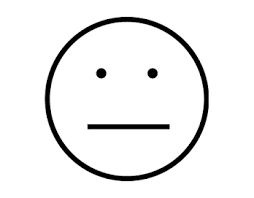
\includegraphics[width=0.5\textwidth]{img/blank.png}
        \caption{Simulated gradient of the thickness mode of the BAW cavity.}
        \label{fig:gradient-dmim}
    \end{figure}

    \section{Proposed Works}
    There are two avenues to be pursued for further development of this WLC scheme. The first is to investigate, through simulation, the relationship between the increase of optomechanical coupling through the application of further silicon nitride coatings and the degradation of the mechanical Q-factor. Secondly, is to probe the experimental details of the implementation of the BAW as a potential candidate for a WLC scheme, namely verify that there exists sufficent coupling for raditiona pressure excite of the mechanical resonance.
    \par
    Details of the mechanical Q-factor of BAW resonators operating at cryogenic temperatures is not particularly novel, however there are many unknowns that may be introduced when applying reflective coatings. Ref \cite{galliou2016} derived an approximate expression to determine the excess mechanical loss induced by thin film coatings and quartz resonators. However, a more systematic approach may be required when applying greater than the single coating to the crystal, as may be required if the single coating does not increase the optomechanical coupling sufficiently. Thus a finite element simulation software such as \texttt{ANSYS} or \texttt{COMSOL} may be required to determine a more accurate estimate of the mechanical Q-factor. This, in conjuction with the previously developed simulations, should enable a more methodical optimisation between the coupling and mechanical Q-factor. 
    \par
    The experimental verification of radiation pressure driving will likely take the majority of efforts within this proposal. There has been previous attempts made to excite a mechanical resonance through the amplitude modulation of the laser within the experimental setup used to take the measurements above. However, this was done using the uncoated resonator as well as in air. Hence the first step will be to place the optical cavity, now containing the coated resonantor, and place it into a vacuum chamber. The vacuum will increase the mechanical Q-factor of the resononator by approximately an order of magnitude (going from $\sim10^5$ in air to $\sim10^6$ in vacuum). Additionally, the use of the coated resonator, with it's doubled optomechanical coupling, will hopefully allow measurement of the radiation pressure driving of the BAW resonantor. If this is not the case, then more coatings of the resonator will be required until thecoupling is sufficent to see this radiation pressure driving. Once this is confirmed, that development of a cryogenic system will begin to take place. This is likely beyond the time frame of a Master's research project, but will be a crucial stage moving forward. The cryogenic system will allow for the move towards the required Q-factor of $\sim10^{10}$ that had been demonstrated in Ref \cite{galliou2013}.

    \section{Conclusion}
    Future gravitational wave detectors will be targeting the high frequency regime, and a serious method for acheiving broadband sensitivity increases is through the use of a WLC scheme. The proposed method for the creation of a WLC scheme is through unstable optomechanical filters, of which the BAW is a potential candidate. The BAW suffers from a low optomechanical coupling and a high resonantor mass, requiring large optical intensities that may introduce excess laser heating. Previously, an increase in this optomechanical coupling has been experimentally demonstrated through the use of reflective coatings, and more importantly, a method of simulating the optomechanical coupling from an arbitrary reflectivity of the BAW was devised. This research is proposed to be focused on two main objectives: to investigate the effect on mechanical Q-factor of the application of further coatings to the BAW through finite element analysis, and to attempt to experimentally measure the radiation pressure excite of the mechanical resonance of the BAW. This second objective will be completed through first placing the existing optical cavity within a vacuum chamber, and then, if need be, applying more silicon nitride coatings to the resonator. 
\end{document}